\title{\textbf{Christian perspectives on sustainability: \\
		The need for numerical answers to philosophical questions.}}
% Sustainability challenges and managing tradeoffs: engineers' need for numerical answers to philosophical questions 
\author{
		% Authors must be italicized.
        \emph{Jeremy Van Antwerp} and \emph{Matthew Kuperus Heun}%
\footnote{
Engineering Department, 
Calvin College,
Grand Rapids, MI, 49546, USA}
}

\documentclass[12pt]{article}

% CEC papers should be set in Times New Roman.
% https://tex.stackexchange.com/questions/153168/how-to-set-document-font-to-times-new-roman-by-command
% suggests the following.
\usepackage{mathptmx}             % For Times New Roman font (or a close approximation thereof).
\usepackage[margin=1in]{geometry} % For 1-inch margins all around.
\usepackage[document]{ragged2e}   % For left justification.
\usepackage{parskip}              % For double-spacing between paragraphs.
\usepackage{nopageno}             % To eliminate page numbers.
% For MLA bibliography. See https://www.ctan.org/pkg/biblatex-mla?lang=en for details.
\usepackage[american]{babel}
\usepackage{csquotes}
\usepackage[style=mla-new]{biblatex}
\addbibresource{JVAMKH.bib}
\usepackage[inline]{enumitem}  % For inline enumerate* lists

\usepackage{titlesec}             % To change formats of section titles, etc.
\titleformat*{\section}{\normalsize}
\titleformat*{\subsection}{\normalsize}
\titleformat*{\subsubsection}{\normalsize}
\titleformat*{\paragraph}{\itshape} % Set paragraph titles to italics
\usepackage{abstract}             % Set characteristics of the abstract
\setlength{\absleftindent}{0in}   % Do not indent left side
\setlength{\absrightindent}{0in}  % Do not indent right side
\usepackage{url}
\setlength{\parindent}{0in}       % Do not indent the 1st line of paragraphs.
\setlength{\parskip}{12pt}        % Instead, add space between paragraphs.
\renewcommand{\abstractnamefont}{\normalfont\normalsize} % Unbold and regular size
\renewcommand{\abstracttextfont}{\normalfont\normalsize} % Unbold and regular size
\date{}                           % To eliminate the date in the title

% To include graphics
\usepackage{graphicx}

% Commands for editing.

\usepackage{xcolor}            % For colored text
\usepackage[normalem]{ulem}    % For \sout command (strikethrough)

% From https://tex.stackexchange.com/questions/130623/crossing-out-using-different-colour,
% Change the \sout color to red
\newcommand{\redsout}{\bgroup\markoverwith{\textcolor{red}{\rule[0.5ex]{2pt}{0.4pt}}}\ULon}

% Use these versions to display changes.
\newcommand{\del}[1]{\textcolor{gray}{\redsout{#1}}}
\newcommand{\ins}[1]{\textcolor{red}{#1}}
\newcommand{\rev}[2]{\del{#1}\ins{#2}}

% Use these versions for a clean copy.
% \newcommand{\del}[1]{}
% \newcommand{\ins}[1]{#1}
% \newcommand{\rev}[2]{#2}



\begin{document}
	
\maketitle

\begin{abstract}
\noindent
\ins{rewrite abstract from scratch. Later.}

\end{abstract}


%%%%%%%%%%%%%%%%%%%%%%%%%%%%%%%%%%%%%%%%%%%%%%%%%%%%%%%%%%%%%%
\section{Sustainability and the disciplines}
\label{sec:sustainability_and_the_disciplines}
%%%%%%%%%%%%%%%%%%%%%%%%%%%%%%%%%%%%%%%%%%%%%%%%%%%%%%%%%%%%%%

Sustainability is challenging because of complexity, scales humans are ill-suited to consider, 
and lack of helpful philosophical and theological frameworks.

Because of circumstances in our world today, 
concerns about environmental, economic, and social 
issues are significant. 
The concept of ``sustainability'' encompasses all three areas
with a view toward the future. 
(See Figure~\ref{fig:3_sustain}.)
One definition of sustainability is
``Sustainability emerges from choices that, on balance, 
promote economic vitality, social equity, and a flourishing natural environment 
both now and for generations to come''~\autocite{Calvin-College-2017}.

Sustainability is considered to be a ``grand challenge,'' 
and becoming more sustainable requires solving 
complex, multidisciplinary, and multifaceted problems
with both technical and non-technical, even philosophical, aspects. 
We engineers design and operate the machines and systems that
%
\begin{enumerate*}[label={(\alph*)}]

  \item generate economic growth by providing employment and economic output, 

  \item enhance society bring people together through communication technologies, and
        
  \item enhance the natural environment.

\end{enumerate*}
%
But we also design machines and systems that
%
\begin{enumerate*}[label={(\alph*)}]

  \item replace human workers,

  \item foster online hate, and
        
  \item consume non-renewable materials and
        emit pollution, thereby contributing to environmental degradation.

\end{enumerate*}
%
Which direction a particular machine or system propels society is a function, in part,
of both its design and of the macro socio-economic policies that inform the design.
Because design is a central function of engineering, 
engineers have an important role to play in determining 
the sustainability of our future. 

But what guides engineers to make design choices that lead to sustainability?
And what guides policy-makers to make socio-economic-environmental
policy choices from which sustainability can emerge?

A traditional answer is ``the academic disciplines,'' 
which are both generators of and repositories for accumulated human knowledge
about a problem domain.
Presumably, academic disciplines can guide design processes for engineers
and policy-making for policy-makers.
Of course, there are academic disciplines 
at each vertex of the sustainability triangle (Figure~\ref{fig:3_sustain}):
Environmental Studies (or Ecology, Biology, etc.) for the Environmental vertex, 
Economics for the Economy vertex, and 
Sociology for the Social vertex.
But sustainability grand challenges exist across disciplinary boundaries and, by definition,
cannot be addressed or solved by a single vertex discipline alone.

\begin{figure}
\centering
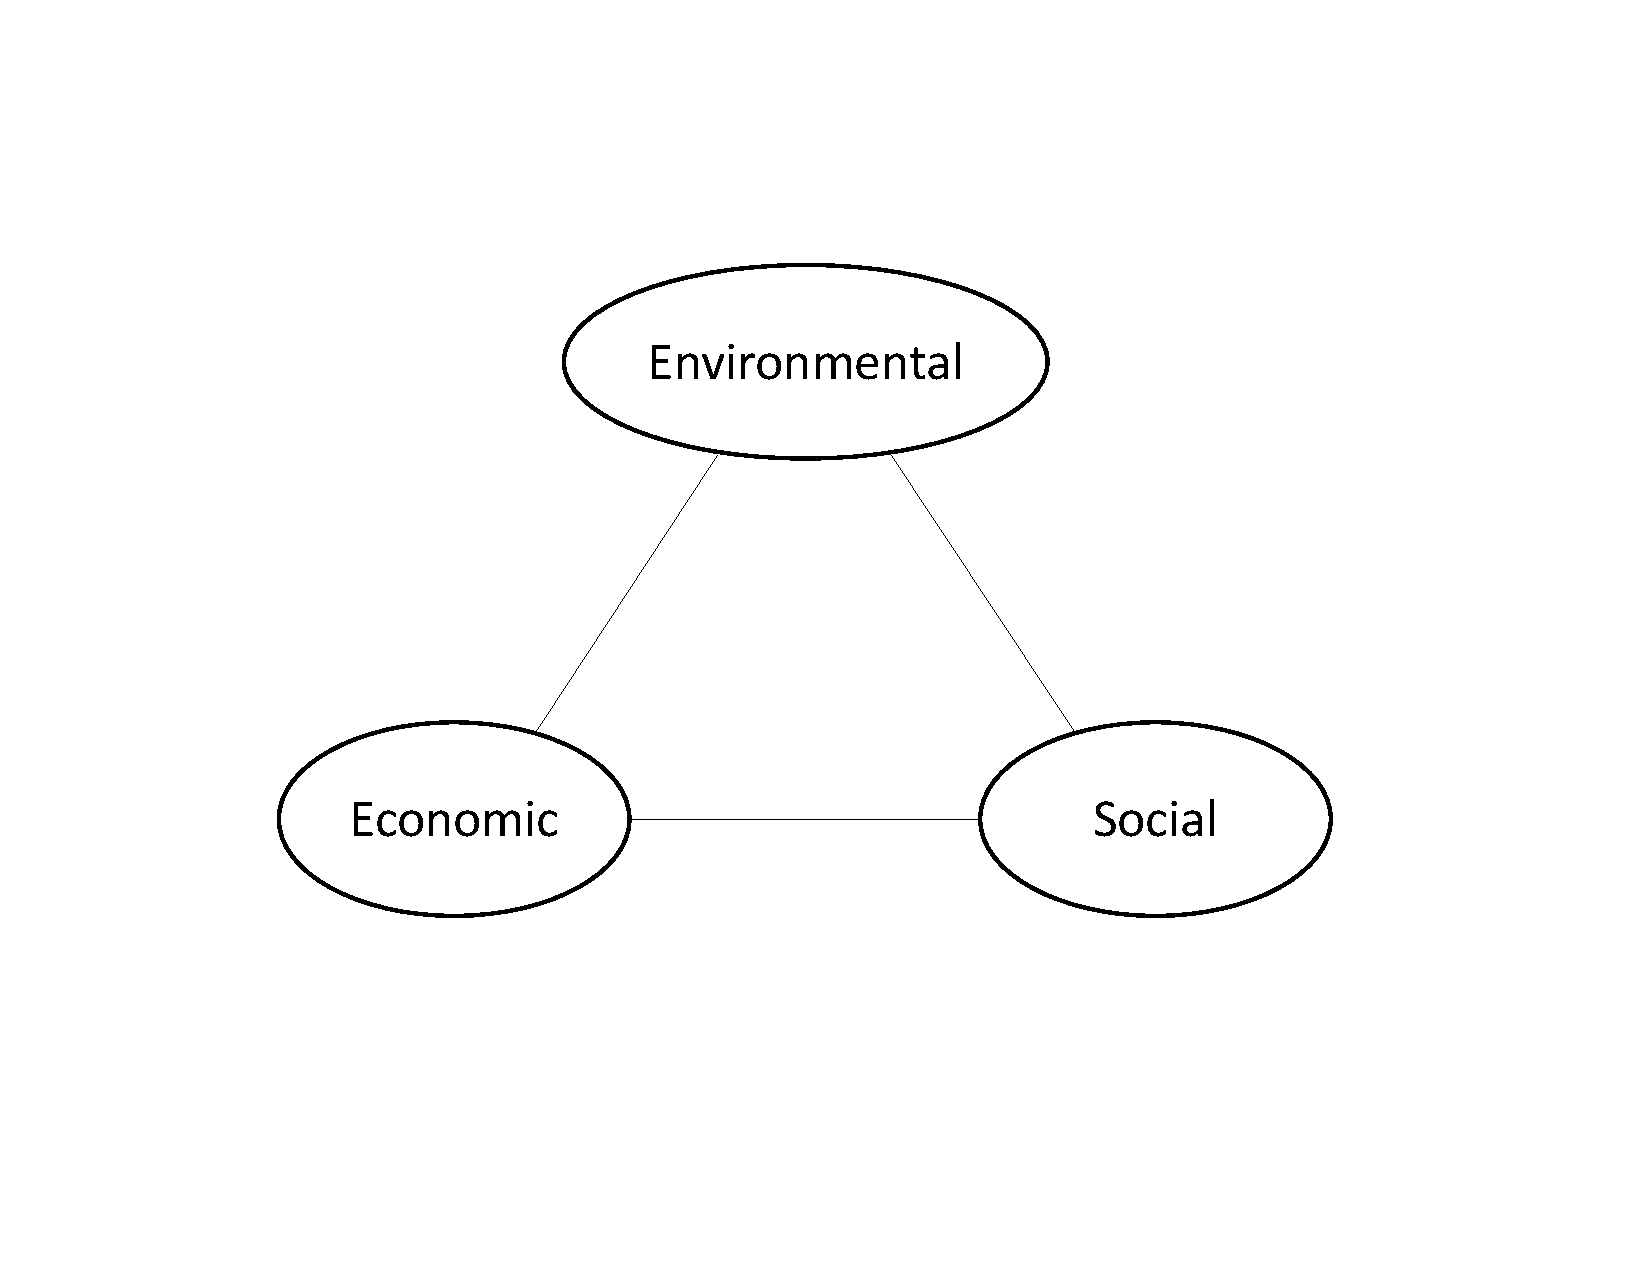
\includegraphics[width=0.75\linewidth]{figure_other/TriangleDiagram.pdf}
\caption{Three aspects of sustainability.}
\label{fig:3_sustain}
\end{figure}

In a hopeful interdisciplinary sign, 
disciplines have emerged along the edges of Figure~\ref{fig:3_sustain}, too.
Environmental Economics was founded in the 1960s,
focusing on valuation of ecosystem services and 
internalizing externalities associated with environmental degradation.
In the 1970s, Environmental Sociology emerged along the Environmental--Social edge 
to study interactions between society and the natural environment. 
Along the Social--Economics edge, Socioeconomics (also called Social Economics) 
emerged in the early 1980s
to study interactions between societies and their economies.
Ecological Economics, founded in the late 1980s, 
emphasizes that the economy as a subsystem of the environment.
There are journals for each edge:
the \emph{Journal of Environmental Economics and Management}, \emph{Ecological Economics}, 
\emph{Environmental Sociology}, 
the \emph{International Journal of Social Economics}, and the \emph{Journal of Socio-Economics}.

However, our assessment of the vertex and edge disciplines,
as presently constituted,
is that they are not policy-relevant
at the macro level. 
For example, these disciplines would focus on the best way to manage a particular forest 
rather than the best way to preserve forests worldwide
in the context of broad economic and social factors.
Furthermore, these edge disciplines exist, almost by definition, 
on the fringes of the vertex disciplines:
E.g., Ecological Economics is not considered ``real'' economics by many economists.
The edge disciplines, by and large, do little to affect the vertex disciplines.

Additionally, what guides Christian engineers to make sustainable design choices
that glorify God and serve humankind
or policy-makers to generate policies that do the same?
One might think that ``Christian Theology'' could provide answers, because
one aspect of theology is discerning the 
ways that deities interact with the natural world. 
However, most Christian thought is focused on interactions among people 
and between individuals and divine beings.

It is rare for Christian theologins to grapple seriously with 
sustainability issues.
We have yet to see sustainability issues engaged in a serious and widespread manner
by Christian theologians and scholars or by denominations.
Thus, to date, there is little indication that Christian Theology 
has provided helpful guidance on sustainability issues
for engineers or policy-makers.


There has been a lot of work in the area of sustainability, but most of it is flawed in one or more ways.
Sometimes sustainability \emph{is} a zero-sum game 
(for instance, you can't \emph{both} use fossil fuels and conserve fossil fuels)
and sometimes sustainability \emph{isn't} a zero-sum game 
(technical innovation sometimes can both improve standard of living and be more energy efficient).
Much of the literature on sustainability assumes that it is possible to have both ``development,'' by which it is meant lifting people out of poverty,
and environmental conservation. 
For example, ``Humanity has the ability to make development sustainable ... widespread poverty is no
longer inevitable if policies that nurture and favor growth are adopted and implemented'' \cite{Ngome2015}.
However, prosperity and conservation are generally at odds. Economic activity requires input of resources
and produces outputs such as pollution. Fundamentally, economic growth is itself unsustainable; at some level of economic activity,
the Earth will not be able to supply the inputs needed and/or absorb the outputs humans produce.

Another common error in the sustainability literature is the assumption that it will be possible to move 
from our current situation to a sustainable future. These studies look forward to an ideal future state without
serious consideration of whether a sustainable future state is practically, physically, and/or technically achievable. 
One helpful question to discern fanciful or wishful thinking in this regards is ``what would have to be true for this to happen?''


%%%%%%%%%%%%%%%%%%%%%%%%%%%%%%%%%%%%%%%%%%%%%%%%%%%%%%%%%%%%%%
\section{Questions}
\label{sec:questions}
%%%%%%%%%%%%%%%%%%%%%%%%%%%%%%%%%%%%%%%%%%%%%%%%%%%%%%%%%%%%%%

\ins{flow from questions to gaps in how Christians think about sustainability.}
Each paragraph ends with a question (in italics) 
--$>$ move the the ends of motivating question 
 We lack tools to give concrete answers to these questions.

\subsection{Social}
For any given level of technological development, there must exist some upper limit to the human population the Earth
can support. Calculating this limit is a technical question and can be technically addressed. The subsequent questions are nontechnical.
\begin{itemize}
\item ``What is the ideal total population?'' (which is less than or equal to maximum possible population) % informed by environmental (and economic?) tradeoffs.
\item ``How should we manage for and arrive at this ideal population?'' and % a means/ends question.
\item ``Where should people live? What is the geographical distribution of population?'' % rights, standard of living = justice.
\end{itemize}
Answers to these questions depend a great deal on \emph{values}. What are the relative preferences for justice, standard of living, 
environmental versus economic and social tradeoffs, and the relative importance of the means versus the end?

What ``right'' do people have to food, water, air, medicine or health care, property, or a ``living'' wage? 
Where do these rights come from? What rights does the nonhuman world have? Where do these rights come from?
What rights do future generations have, and where do their rights come from? % love your neighbor as yourself?
When tradeoffs exists between these rights, how do we manage resolution?
How do/should Christian assessments of tradeoffs change when cost and benefits fall to different (groups of) people?
Does it depend on whether many benefit at the expense of a few of if few benefit at the expense of many? 
When benefits and costs accrue to different generations? 
Does the size of the benefit/cost matter? 
Does the number of people in the group matter? Surely, it must but what is a ``large enough'' difference to matter?

Regarding gloomy predictions about sustainability issues, such as climate change, global population,
or in terms of world energy supply, there are those who will say ``don't worry, it will all work out,'' while
others respond ``no it won't.'' Who should we give credence to? Obviously, those who are telling the truth. But that can
be hard to identify. (The Old Testament criteria for determining the legitimacy of a prophet comes to mind, but the
Israelites had a poor track record of following prophetic advice.) There are technical truths and moral truths. Should
the opinion of an expert researcher or technologist count for more than a blue-collar ``man on the street?'' How about a
government leader? Does it matter if the question under consideration is technical or nontechnical?

\subsection{Social economics}

A policy-driven change, such as reducing carbon emissions by banning air travel, results in consequences that have
\emph{direct} dollar-measurable impacts (such as change in GDP), \emph{indirect} but still dollar-measurable
consequences (such as reduced CO$_2$ output), and consequences that \emph{aren't} measurable in dollars (such as an
aesthetic impact on the landscape). Economic cost-benefit analysis converts all social and environmental costs to
dollars, thereby providing a consistent numeraire and allowing direct comparisons among environmental, economic, and
social effects. How should Christians evaluate choices among policy solutions whose impacts are dollar-quantifiable and
those that are \emph{not} dollar-quantifiable? 

\subsection{Environmental social justice}
How do Christians balance stewardship of the natural world with loving our neighbor?
Both the Old and New Testaments teach that Christians should work to eliminate poverty. 
How do we respond to the observation that alleviating poverty increases economic consumption, which has negative environmental consequences?
Suppose a third-world farmer argues that he/she needs to make a living. 
Can he/she create another subsistence farm via slash-and-burn agriculture in the rainforest?  
It could be argued that it is sinful \emph{not} to make use of a resource, such as coal or petroleum. 


\subsection{Environmental economics}
There are those who say that coal mining is good because the benefit of employment in the coal industry outweighs
any (potential) environmental harm caused from mining and burning coal. How large does the cost-benefit differential
have to be for this to be true? This is an entirely practical question that demands a concrete, numerical answer.

Some consequences of a ban on air travel would include the destruction of the air travel industry and its ancillary
industries. How does the weighing of tradeoffs (e.g., economic versus environmental) differ if the loss of jobs is not
the result of a regulation, but instead comes from technological innovation or market forces? Should this make a
difference? Does it?

\subsection{Multifaceted sustainability}
In 2013, air travel was responsible for about 3\% of US greenhouse gas emissions. % citation needed. EPA data appears to be offline now.
% see https://www.c2es.org/content/reducing-carbon-dioxide-emissions-from-aircraft/
% which cites Inventory of U.S. Greenhouse Gas Emissions and Sinks: 1990–2015 (U.S. Environmental Protection Agency, 2017)
Air travel is a particularly \emph{carbon intensive} activity. Therefore, banning air travel would be a step to making the 
world a more sustainable place. Engineers are well equipped to analyze some of the effects of this proposal. For instance,
engineers could estimate the resulting \emph{increase} in emissions from other forms of transportation that would result from 
the ban on air travel. However, \emph{how should the social and economic consequences be weighed against the environmental 
benefits}? What is the balance between the needs to the present and the needs of the future?	
Do economic, social, and environmental factors weigh differently in that decision?	

Banning air travel might be considered a ``clean'' or ``ideal'' policy option. Other policy options could be classified
as pragmatic, such as improving air travel energy efficiency. How should Christians navigate the space between ideal and
pragmatic policy proposals?



As a society, we have \emph{de facto} arrived at answers to questions such as the ones above. However, 
there is increasing reason to believe that the answers we have are not the answers that will lead to a sustainable future.
Moreover, the hows and whys of the answers that we have need to be reexamined.
\ins{Need a concluding and/or summarizing statement. Something along the lines of ``thus, it's clear that we lack the theological
and philosophical framework that would allow us to to address sustainability issues.''}

% Add: Utilitarian/Kantian ethics? Engineers like these because they allow us to calculate the greatest good for the greatest number of people.
% If an answer is mathematical, it must be true.


%%%%%%%%%%%%%%%%%%%%%%%%%%%%%%%%%%%%%%%%%%%%%%%%%%%%%%%%%%%%%%
\section{The need for a theology of sustainability}
\label{sec:need_for_theology_of_sustainability}
%%%%%%%%%%%%%%%%%%%%%%%%%%%%%%%%%%%%%%%%%%%%%%%%%%%%%%%%%%%%%%





%%%%%%%%%%%%%%%%%%%%%%%%%%%%%%%%%%%%%%%%%%%%%%%%%%%%%%%%%%%%%%
\section{Worldviews}
\label{sec:worldviews}
%%%%%%%%%%%%%%%%%%%%%%%%%%%%%%%%%%%%%%%%%%%%%%%%%%%%%%%%%%%%%%


%++++++++++++++++++++++++++++++
\subsection{Environmental Perspectives}
\label{sec:environmental}
%++++++++++++++++++++++++++++++

The book \emph{Ecologies of Grace} \autocite{Jenkins:2008}
provides a topology of Christian thought regarding the 
nonhuman creation and the
environmental aspect of sustainability.
He identifies three schools of thought:
stewardship, 
eco-justice, and 
ecological spirituality,
which loosely correspond to 
Reformed (or evangelical protestant), 
Roman Catholic, and 
Eastern Orthodox 
traditions.
To Jenkins' three, we add a fourth:
consumptive economic prosperity and
the conservative evangelical tradition. 
These four schools of thought 
span a wide range of Christian stances toward the nonhuman creation
and 
consequently outline a range of possibilities 
for Christian responses to environmental issues
and environmental sustainability concerns more broadly.
One way to begin unpacking the four schools of thought 
is to identify a keyword for each:
\emph{redemption} for stewardship, 
\emph{sanctification} for eco-justice,
\emph{deification} for ecological spirituality, and
\emph{resilience} for consumptive economic prosperity.

%..............................
\paragraph{Redemption} 
\label{sec:redemption}
%..............................

The stewardship school of thought in the Reformed tradition
emphasizes that all of human existence
is a response to God's redemptive acts
and God's providence to humans.
Knowing God leads to vocational responsibility 
to care for nonhuman creation,
the means by which God provides for humankind  % ==== telos?!
% For some reason, we need to include this citation twice to get both author and page number to appear.
(\textcite{Jenkins:2008} \textcite[19]{Jenkins:2008}). 
Thus, all human work to care for the creation 
is seen as service to the Creator
out of gratitude for redemption (\textcite{Jenkins:2008} \textcite[77]{Jenkins:2008}).
\emph{Earthkeeping} \autocite{Wilkenson:1980aa} provides a cogent summary
of the importance of redemption for Reformed Christians doing creation care.

The idea of stewardship is a reaction against themes of human dominion over the nonhuman creation
that emerge from some interpretations of the creation stories in Genesis.
Christians in this tradition are inspired by an interpretation of Gen~1:26–28 in which 
``the proper exercise of dominion yields shalom: the flourishing of all creation'' \autocite{BoumaPrediger:2019}.
As such, the first order of business for stewardship-minded Christians
is to act as shalom-building caretakers of God's creation.

The \emph{stewardship} viewpoint acknowledges that tradeoffs
are present in every policy and in every decision. 
So, in an engineering sense, 
Christian environmental stewardship could be considered an optimization problem
in which policies that bring about the most good 
are to be preferred.
Designs and policies can be critiqued based on the \emph{process} by which they emerged.
Were all voices heard? Was the assessment of tradeoffs accurate?
Who decides what goods matter most is important, and 
all voices should be heard on each matter.
Ignoring or disregarding voices is dangerous,
since injustices could result.
Humans will be persuaded on the right course of action
for sustainability policies by weighing the tradeoffs 
among environmental, economic, and social factors.

Weakness of this approach are
%
\begin{itemize}

  \item deliberation needs to be exhausgive and can be exhausting

  \item imperfect informaiton can lead to disasterous results.

\end{itemize}


%..............................
\paragraph{Sanctification} 
\label{sec:sanctification}
%..............................

The eco-justice school of thought in the Roman Catholic tradition
emphasizes that God's grace reveals the creation's 
inherent integrity \autocite[19]{Jenkins:2008}, 
giving it natural value and inherent moral standing~\autocite{Joldersma:2019}. 
Thus, Christians must respect creation's inherent value and 
respond to its moral standing in all activities.
If the nonhuman creation can't speak for itself, 
we must speak for it and defend it when necessary.

The \emph{Laudato Si} encyclical \autocite{Pope-Francis:2015aa} 
is a clear enunciation of Roman Catholic thought
on environmental sustainability issues.
In it, Pope Francis portrays the nonhuman creation as a
``sister with whom we share our life and a beautiful mother who opens her arms to embrace us''
(\textcite{Pope-Francis:2015aa} \textcite[3]{Pope-Francis:2015aa}).
However, our sister and mother
``cries out to us because of the harm we have inflicted on her 
by our irresponsible use and abuse of the goods with which God has endowed her''
(\textcite{Pope-Francis:2015aa} \textcite[3]{Pope-Francis:2015aa}).
With this framing, the Holy Father evokes centuries of Catholic social teaching
about the need to support the oppressed, the poor, and the vulnerable.
Christians in the eco-justice tradition would point to the beatitudes (Lk 6) 
for reminders of the inherent value of those who are oppressed.
The first order of business for eco-justice-minded Christians
is to bring justice to the nonhuman creation, to right the wrongs
of abuse that humans have heaped upon the nonhuman creation.
\ins{this is the ends. What about the means?}

The eco-justice point of view
would weigh the environmental justice of any design or policy
against the possible economic injustice of depriving others
(especially the poor). 
Eco-justice adherents would be more likely to approve a design or support a policy if it
were accompanied by a robust and reliable way to ensure that one people group or another
are not disproportionally affected.

Furthermore, eco-justice is based upon the moral standing of the nonhuman creation,
meaning that the nonhuman creation itself must be given a voice.
To properly evaluate sustainability tradeoffs,
someone must be empowered to speak for the nonhuman creation and
give voice to unjust and unfair aspects of policies and decisions
that have implications for sustainability and the nonhuman creation.
Humans will pursue the right course of action on sustainability issues
when someone speaks eloquently and forcefully for the
those who can't speak for themselves, including the nonhuman creation.


%..............................
\paragraph{Deification} 
\label{sec:deification}
%..............................

The deification school of thought in the Eastern Orthodox tradition
highlights the union between all of creation and God.
Consequently, and by virtue of both owing their existence to the creator,
there is a radical connectedness among all human and nonhuman creatures 
in the creation~\autocite[93]{Jenkins:2008}.

The speech ``To Commit a Crime Against the Natural World Is a Sin'' 
\autocite[133-136]{Bartholomew-I-of-Constantinople:2011aa}
provides an excellent summary of the Eastern Orthodox view
on the nonhuman creation.
In it, Bartholomew states,
``at the heart of the relationship between man and environment 
is the relationship between human beings.
As individuals, we live not only in vertical relationships to God 
and horizontal relationships to one another, but 
also in a complex web of relationships that extend throughout
our lives, our cultures, and the material world.''
(\textcite{Bartholomew-I-of-Constantinople:2011aa} 
\textcite[133--134]{Bartholomew-I-of-Constantinople:2011aa})
Thus, any harm done to the nonhuman creation is a harm done to other human being, but
any good done to the environment is a good done to humans, 
and praiseworthy. 
In the ``ecological spiritualities'' school of thought, 
tradeoffs between the environmental and economic and social realms of sustainability
fade into the background. 
And because the economy is a way of organizing social relationships and structures,
tradeoffs between the environmental and economic are minimized, too.

The first order of business for Christians in the ``ecological spiritualities'' mindset 
is asceticism, self-restraint for the good of the nonhuman creation and for others.
Asceticism will lead to practices that look much like conservation of the nonhuman creation.




%..............................
\paragraph{Resilience} 
\label{sec:resilience}
%..............................

The resilience school of thought in the conservative evangelical tradition
holds that the nonhuman creation is resilient, robust, and self-correcting.
Furthermore, its well-being is assured by God because part of the ``goodness'' that God design into the world is robustness to human action.
God is always in control.
In this school of thought, human well-being is paramount. 
Thus, humans are to be consumers of the nonhuman creation 
to provide economic prosperity and
lift people out of poverty.
Documents from the Cornwall Alliance 
provide a summary of conservative evangelical thinking on creation care issues
\autocite{Cornwall:2006aa}.


%++++++++++++++++++++++++++++++
\subsection{Economic and Social Perspectives}
\label{sec:economic_and_social}
%++++++++++++++++++++++++++++++

\begin{figure}
\centering
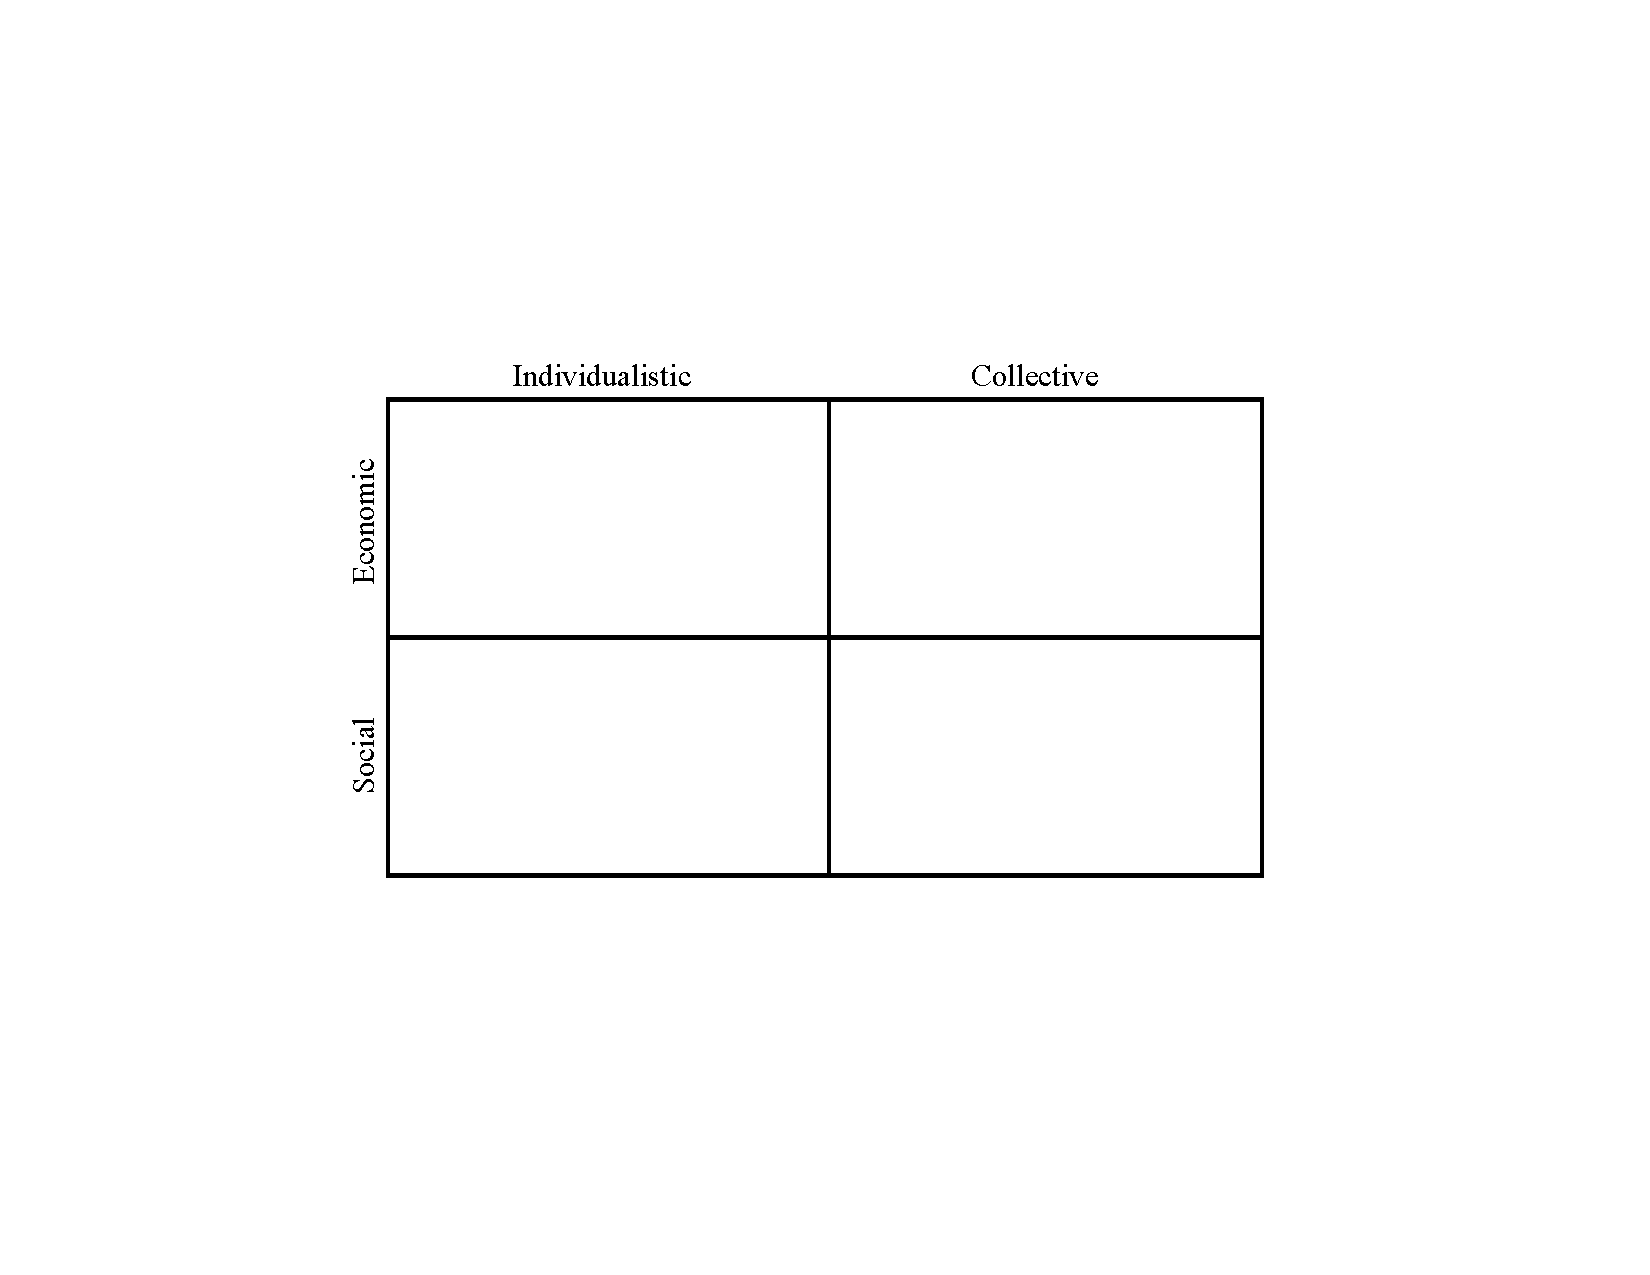
\includegraphics[width=0.75\linewidth]{figure_other/QuadTable}
\caption{Table for individualistic and collectivistic views on economic and social issues.}
\label{fig:table}
\end{figure}

% Need to refer to the figure. Need to harmonize/standardize terminology. I suggest ``individual'' and ``collective'' and the ``-ivistic'' ending.
% Need to note that these cut across, to some degree, the ``Christian'' axis. 

The economic and social aspects of sustainability are inextricably linked. Biblical teaching on money
and justice are often recognized as two sides of the same coin, for instance in Micah 2:1-2, where the unjust deeds that
are denounced are economic in nature. Biblical teaching on economics and justice tends not to be in terms of a
systematic, over-arching theory, but rather in terms of individual interactions.
One exception to this pattern is the Old Testament sabbatical/jubilee system of canceling debt and returning property. 
In modern economic terms, canceling debts and returning property would serve to minimize 
\emph{income inequality} and ensure that there was universal access to the \emph{means of production}.
% Insert Matt's really important comment here.

From the first chapter of Genesis, the call to stewardship has
been understood by Christians to include money. The power of earthly resources to accomplish ``heavenly things'' is made
explicit in the parable of the shrewd (or dishonest) manager in Luke 16. To this end, the great majority of the Bible's
teaching on money relates to generosity to the poor. Numerous Old and New Testament passages instruct God's faithful to
give generously to the poor, the disadvantaged, and the marginalized, where ``giving'' is some combination of money
(traditionally called ``alms''), material goods (such as food or clothing), and justice or fairness.

One branch of Christian thought views wealth itself as a root of evil. This view goes beyond merely \emph{love} money
being the root of evil (I Tim 6:10). Proponents of the view that money itself is a source of evil would point to Jesus
telling the rich young man to sell all his possessions and give to the poor and Jesus' further comment that it is easier
for a camel to go through the eye of a needle than for a rich man to enter the kingdom of God (Mt 19:16-30, Mk 10:17-31,
Luke 18:18-30). At the other end of the spectrum of Christian thought, worldly wealth is seen as God's blessing, even an
indication of his favor (in a more extreme version of this view).

In terms of modern economic views, Christians hold a wide range of positions. Some Christian traditions advocate a
communal economic arrangement, in imitation of the early church (Acts 2:42-46). Examples range monastic orders such as
might be found in Roman Catholic or Eastern Orthodox traditions to the Hutterite and Bruderhof communities, which come
from an Anabaptist tradition. At the other end of the economic spectrum, many Christians advocate for an economic system
based on individual ownership and freedom of enterprise. Some key verses that support a more individual view include the
comments ``Didn’t it belong to you before it was sold? And after it was sold, wasn’t the money at your disposal?'' (Acts
5:4) and Paul's instruction that we should work to eat (2 Thes 3:10) and to share with those in need (Eph 4:28).
Thus, Christians hold a range of views from economic thought from communalistic to individualistic.

Likewise, Christian social perspectives can stress individual freedom or collective behavior
A liberal approach to providing for poor widows would be represented by the instruction that widows should be 
provided for, first of all, from their own families (1 Tim 5:4). 
The collective approach is represented by the group effort of caring for widows at the beginning of Acts chapter 6.
Denominational polity is another example of the individual-to-collective spectrum.
At the individual end of the spectrum are ``independent'' churches that recognize no higher authority than the congregation itself.
In the middle are denominations that follow a presbyterian form of church 
government. The local church in the presbyterian system has some autonomy but within the constraints of the broader 
denominational structure. The local churches also have a voice in the operation of the collective. At the collective end of the spectrum 
are denominations that use an episcopal form of church government. Denominations with an episcopal polity operate in a very ``top down'' 
way.

We next show how the individualistic/collectivistic economic and social (that is, political) perspectives apply to a solving sustainability problems.

\subsection{Christian solutions to the tragedy of the commons}
\label{sec:totc}
The term ``tragedy of the commons'' was popularized by Hardin \autocite{Hardin68} 
and is used as a shorthand way of referring to
situations where there is equal and open access to a resource or pool of resources and it is in the rational self-interest of
every individual to maximize their use of the resource, even if this results in the net effect of destroying the
resource itself through over exploitation. This class of problems is recognized as ``having no technical solution.''
Instead, sustainable solutions are the result of social and/or economic policies. This section will examine several
Christian responses to the tragedy of the commons.

As originally stated, each herdsman had incentive to add more animals to his flocks grazing on the common land, since
the benefits (the extra animals) would accrue solely to him but the cost (degradation of the land) would be split between
all herders using the land for grazing. Moreover, since he knew that every other herder faced the same set of
incentives, it is rational to predict that the land will be ruined and that he should ``get while the getting is good.''
The ``tragedy'' lies in the ``remorseless working out of things.''

One collectivistic solution to the tragedy of the commons is for all of the animals grazing on the commons to be common
property. Every member of the community would receive an equal share of the common herd (for example, cash value of the
meat raised at the end of the year). It would thus be in every individual's self-interest to maximize the \emph{total}
output, not just their own output. An individualistic solution is to charge each herder an increasing amount of rent for
each additional animal placed on the common land, which would create a financial incentive for each herdsman to keep
only a reasonable number of animals on the common land. A liberal social solution would be for each herder to be allowed
only a limited number of animals on the common land. A collective solution would be where an authoritative governing
board is set up to administer the common land. The board decides how many animals total are allowed and what proportion
of that total is allocated to each individual herdsman.

As we'll see below, many sustainability challenges are wholly or partly ``without technical solution'' and we need
Christian approaches to solving these problems.






%%%%%%%%%%%%%%%%%%%%%%%%%%%%%%%%%%%%%%%%%%%%%%%%%%%%%%%%%%%%%%
\section{Conclusions}
\label{sec:conclusions}
%%%%%%%%%%%%%%%%%%%%%%%%%%%%%%%%%%%%%%%%%%%%%%%%%%%%%%%%%%%%%%



\printbibliography
\end{document}